\section{Neural Networks: Representation}

    \subsection{Non-linear Hypothesis}
        \begin{itemize}
            \item Example: non-linear classification- logistic regression has lots of terms and not scalable( $O(n^2), O(n^3)$).
            \item Application: computer vision
            \item Neural network is useful for \textbf{non-linear, large scale classification}.
        \end{itemize}

    \subsection{Neurons and the brain}
        \begin{itemize}
            \item Origin: neuromorphic computing mimics how brain functions.
            \item Recent resurgence due to hardware advancement.
            \item The ``one-learning hypothesis'': there exists a single algorithm that the brain uses for generalized learning. 
                \begin{itemize}
                    \item Neural re-wiring: wiring the auditory cortex to eyes, then the cortex learns how to \emph{see}.
                \end{itemize}
        \end{itemize} 


    \subsection{Model representation}
        \begin{figure}[htbp]
            \centering
            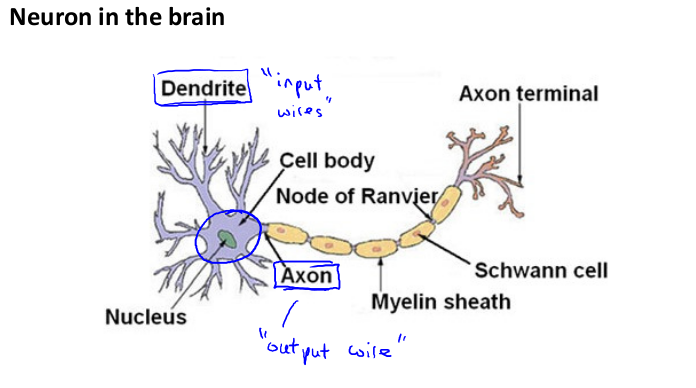
\includegraphics[width=\textwidth]{image/neuron.png}
            \caption{A biological neuron}
            \label{fig:neuron}
        \end{figure}

        Figure \ref{fig:neuron} shows a model of a biological neuron. The \textbf{dendrites} are the wires which receive input signal. The \textbf{axons} output the signal.

        \subsubsection{Neural model: logistic unit}
            In our model:
            \begin{itemize}
                \item Dendrites: input features x\textsubscript{1}, x\textsubscript{2}, \dots, x\textsubscript{n}.
                \item Output: result of hypothesis function.
                \item x\textsubscript{0}: bias unit (:= 1).
                \item Logistic function: $\frac{1}{1+exp(-\theta^T X)}$, referred to as the sigmoid(logistic) \textbf{activation} function.
                \item $\theta$ are referred to as \textbf{weights}.
            \end{itemize}

            Visually, a simplistic representation can be view as 

            \begin{equation}
                [x_0\; x_1\; x_2]\: --> \: [\:]\: -->\: h_\theta (x)
                \label{fig:visual-nn-repr}
            \end{equation}


            The input nodes (layer 1, input layer) go into the another node (layer 2), which then outputs to hypothesis function (output layer).

            In this example, we label the intermediate layers of nodes (between the input and output layers) $a^2_0, \dots, a^2_n$: \textbf{activation units}. 
            Definitions:\\

            \fbox{
                $ a_i^{(j)} $ = ``activation of unit i in layer j 
            }\\

            \fbox{
                $\Theta^{(j)}$= matrix of weights controlling function mapping from layer j to layer j+1.
            }\\
          
            If we had one hidden layer, it would look like:

            \[
                \boxed{
                [x_0 \, x_1 \, x_2\, x_3] \:--> \: [ a_1^{(2)},a_2^{(2)},a_3^{(2)}] \: --> h_\theta (x)
            }
            \]  
    
            The value for each of the activation node is obtained as follows;

            \[
                a_1^{(2)} = g (\Theta^{(1)}_{10} x_0 + \Theta^{(1)}_{11} x_1 + \Theta^{(1)}_{12} x_2+\Theta^{(1)}_{13} x_3 )
            \] 

            \[
                a_2^{(2)} = g (\Theta^{(1)}_{20} x_0 + \Theta^{(1)}_{21} x_1 + \Theta^{(1)}_{22} x_2+\Theta^{(1)}_{23} x_3 )
            \] 

            \[
                a_3^{(2)} = g (\Theta^{(1)}_{30} x_0 + \Theta^{(1)}_{31} x_1 + \Theta^{(1)}_{32} x_2+\Theta^{(1)}_{33} x_3 )
            \] 

            \[
                h_\Theta(x) = a_1^{(3)} = g (\Theta^{(1)}_{10} a_0 + \Theta^{(1)}_{11} a_1 + \Theta^{(1)}_{12} a_2+\Theta^{(1)}_{13} a_3 )
            \] 

            Essentially, each layer j has its own \textbf{matrix of weights}, $\Theta^{(j)}$. \textbf{If network has $s_j$ units in layer j and $s_{j+1}$ units in layer j+1, then $\Theta^{(j)}$ will be of dimension $s_{j+1} \times (s_j +1)$.} The +1 comes from the addition in $\Theta^{(j)}$ of the bias nodes, $x_0$ and $\Theta_0^{(j)}$. 

            Example: if layer 1 has 2 input nodes and layer 2 has 4 activation nodes- dim ($\Theta^{(1)}$) is going to be 4x3 where $s_j=2$ and $s_{j+1}=4$, so $s_j+1\times (s_j +1)=4\times3$.

